\documentclass{article}
\usepackage[utf8]{inputenc}
\usepackage{amsmath}
\usepackage{amssymb}
\usepackage{enumitem}
\usepackage[hidelinks, pagebackref=true]{hyperref}
\usepackage{multicol}
\usepackage{authblk}
\usepackage{biblatex}
\usepackage{multirow}
\usepackage{mathtools}
\usepackage{float}
\usepackage{multicol}
\usepackage{graphicx}
\restylefloat{table}
\usepackage{caption}
\usepackage{subcaption}
\usepackage{caption, floatrow}
\usepackage{mathrsfs}
\usepackage{hyperref}
\usepackage{epstopdf}
\usepackage[margin=0.5in]{geometry}
\epstopdfDeclareGraphicsRule{.gif}{png}{.png}{convert gif:#1 png:\OutputFile}
\AppendGraphicsExtensions{.gif}

\newtheorem{definition}{Definition}
\newtheorem{lemma}{Lemma}
\newtheorem{sublemma}{Lemma}[lemma]
\title{Domain Prompt Learning for Efficiently Adapting CLIP to Unseen Domains}

\author[1]{Xin Zhang}
\author[1,2]{Shixiang Shane Gu}
\author[1]{Yutaka Matsuo}
\affil[1]{The University of Tokyo}
\affil[2]{Google Research, Brain Team}



\addbibresource{resource.bib}
\begin{document}

\maketitle
\subsection*{Abstract}
Domain generalization (DG) is a difficult transfer learning
problem aiming to learn a generalizable model for unseen domains. Recent foundation models (FMs) are robust to many
distribution shifts and, therefore, should substantially improve the performance of DG. In this work, we study generic
ways to adopt CLIP, a Visual-Language Foundation Model,
for DG problems in image classification. While ERM greatly
improves the accuracy with bigger backbones and training
datasets using standard DG benchmarks, fine-tuning FMs
is not practical in many real-world situations. We propose
DPL (Domain Prompt Learning) as a novel approach for domain inference in the form of conditional prompt generation.
DPL achieved a significant accuracy improvement with only
training a lightweight prompt generator (a three-layer MLP),
whose parameter is of equivalent scale to the classification
projector in the previous DG literature. Combining DPL with
CLIP provides surprising performance, raising the accuracy
of zero-shot CLIP from 73.7% to 79.3% on several standard
datasets, namely PACS, VLCS, OfficeHome, and TerraIncognita. We hope the simplicity and success of our approach
lead to broader adoption and analysis of foundation models
in the domain generalization field. Our code is available at
https://github.com/shogi880/DPLCLIP


\section{Introduction}
Pre-training large vision models using web-scale images is
an essential ingredient of recent success in computer vision. Fine-tuning pre-trained models, such as ResNet (He
et al. 2015) and Vision Transformer (ViT) (Dosovitskiy et al.
2020) is the most popular paradigm for many downstream
tasks. However, domain shifts pose a substantial challenge
in real-world scenarios for successfully transferring models.
Over the past decade, various studies on domain generalization (DG) have sought a systematic way to narrow the gap
between source and target domains (Zhou et al. 2021a; Wang
et al. 2021; Shen et al. 2021) aiming to build a model that
generalizes to unseen domains. Despite the significant work
on this front, machine learning systems are still vulnerable
to domain shifts even after using DG methods (Gulrajani and
Lopez-Paz 2020).
Large pre-trained vision-language models like Contrastive Language-Image Pre-Training (CLIP) are an emerging category of models showing great potential in learning


See the image in figure \ref{fig:my_label1}
\begin{figure}
    \centering
    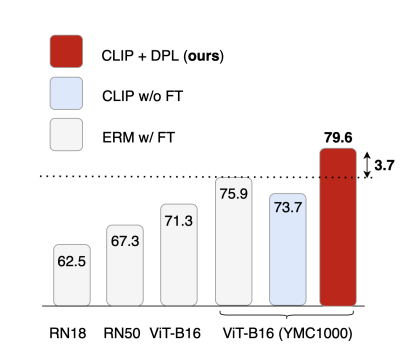
\includegraphics[width=0.95\linewidth]{figure1.jpg}
    \caption{Caption}
    \label{fig:my_label1}
\end{figure}

See the image in figure \ref{fig:my_label2}
\begin{figure}
    \centering
    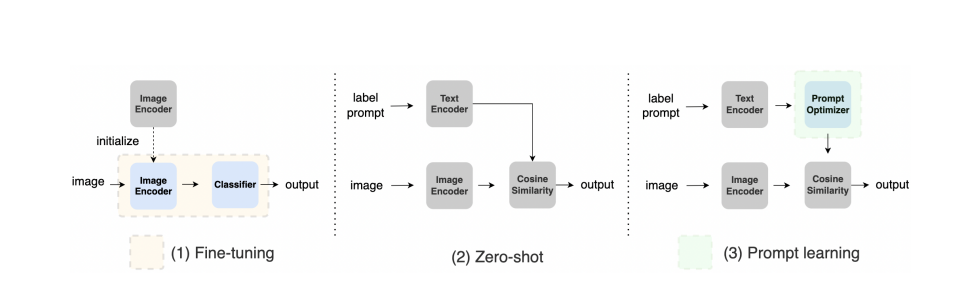
\includegraphics[width=0.95\linewidth]{figure2.jpg}
    \caption{Caption}
    \label{fig:my_label2}
\end{figure}


\section{Method}

In this section, we first introduce the notations and definitions of DG following (Wang et al. 2021). Then, we explain how to use CLIP in DG and introduce Domain Prompt
Learning to enhance CLIP performance in DG.
\subsection{Problem Setup of DG}
See the image in figure \ref{fig:my_label3}
\begin{figure}
    \centering
    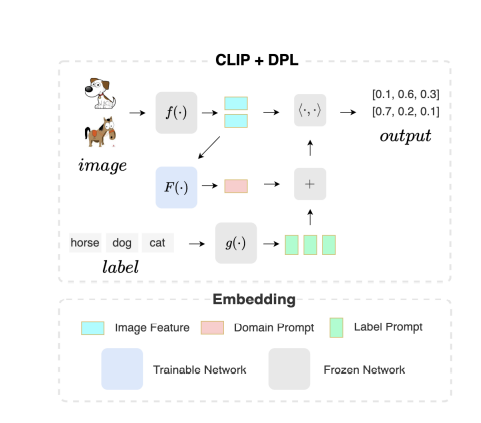
\includegraphics[width=0.95\linewidth]{figure3.jpg}
    \caption{Caption}
    \label{fig:my_label3}
\end{figure}
\begin{equation}
    x = \frac{\sqrt{\sin{\theta}} + {\cos{\theta}} + T_i }{e^{-20}}
\end{equation}

\begin{equation}
    1 + 2 + 3 + \dots + n = \frac{n(n+1)}{2} = \sum_{i = 1}^{i = N} i
\end{equation}
\subsection{Na¨ıve Approaches for Using CLIP in DG
}



\subsection{Domain Prompt Learning for CLIP in DG
}


\section{table}
\begin{table}[]
    \centering
    \begin{tabular}{|c|c|c|}
    \hline
         \multicolumn{2}{|c|}{}sta& &\multicolumn{2}{|c|}{}sta \\
         \hline
         \multicolumn{2}{|c|}{1}& 4\\
         \hline
         & & \\
    \hline
    \end{tabular}
    \caption{Multiple table}
    \label{tab:multitable}
\end{table}







\section{Conclusion}
We introduce CLIP to DG on DomainBed. For this purpose,
we proposed a novel approach called Domain Prompt Learning (DPL) for efficiently adapting CLIP to an unseen domain. By generating the domain prompt conditional on input images, CLIP + DPL brings substantial improvements
over strong DG baselines and several effective TTA methods on DomainBed. Then, we conducted ablation experiments with various backbones and Frozen ERM. We verified
that DPL can stabilize performance and present meaningful
insights about existing datasets and fine-tuning strategy of
backbones. We hope that our research will broaden and inspire the roles of prompt learning in domain transfer learning

\subsection{Limitation}


Interpretability of Domain Prompt To better perform,
our DPL is directly represented in a continuous vector
form, which lacks interpretability. However, improving interpretability is an important research direction in both FM
applications and Domain Generalization. We consider producing discrete semantically informative prompts by some
means is an exciting extension of DPL, even with some loss
of precision.
Label Shift From the technical perspective, DPL cannot
capture the domain shift outside of the images because
DPL uses domain features extracted from only images. As a

\subsection{Future Work}
First and foremost, interpretability is critical in both Domain
Transfer Learning and the Foundation Model. As discussed
in subsection 5.1, DPL introduce the possibility of using a
large language model in DG in the form of prompt. We will
investigate this direction in our future work.
There are two simple and critical approaches to improving
the performance of DG. One is to apply visual prompt tuning (Jia et al. 2022) on the pure visual backbones, which can
be used to more previous methods. Another is focusing on a
data-centric approach since we observe uneven data quality
on the widely used datasets.
Finally, several recent studies systematically analyze the
performance and shortcomings of large-scale pre-train models in the Out-of-Distribution generalization (Cha et al.
2022; Wenzel et al. 2022). We hope that our results will inspire more research in this direction
\section{appendix}

See the image in figure \ref{fig:my_label4}
\begin{figure}
    \centering
    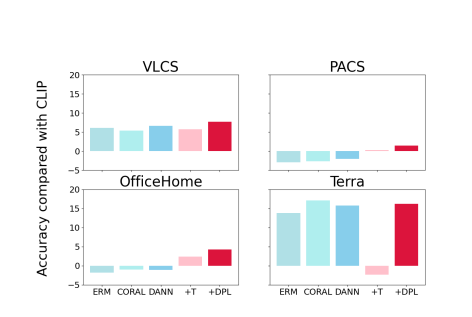
\includegraphics[width=0.95\linewidth]{figure4.jpg}
    \caption{Caption}
    \label{fig:my_label4}
\end{figure}

See the image in figure \ref{fig:my_label5}
\begin{figure}
    \centering
    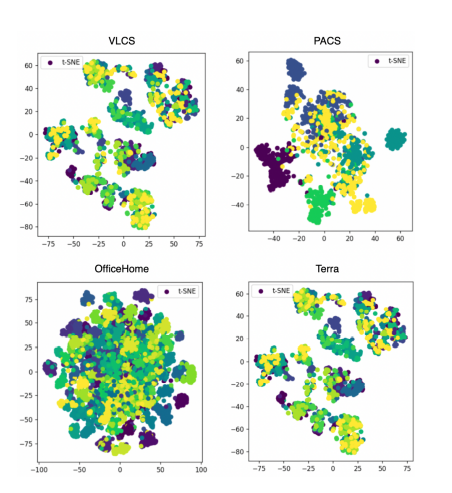
\includegraphics[width=0.95\linewidth]{figure5.jpg}
    \caption{Caption}
    \label{fig:my_label5}
\end{figure}




See the image in figure \ref{fig:my_label6}
\begin{figure}
    \centering
    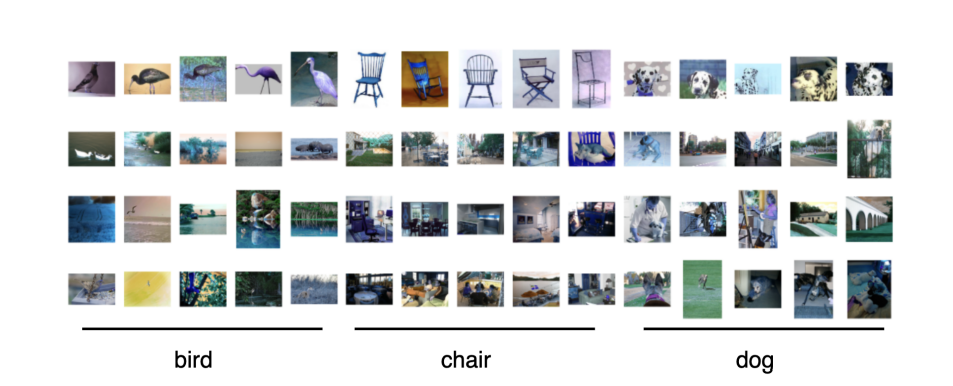
\includegraphics[width=0.95\linewidth]{figure6.jpg}
    \caption{Caption}
    \label{fig:my_label6}
\end{figure}




See the image in figure \ref{fig:my_label7}
\begin{figure}
    \centering
    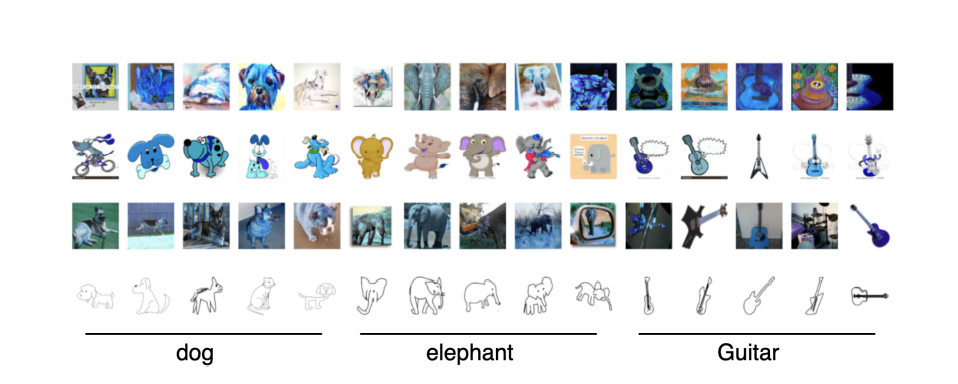
\includegraphics[width=0.95\linewidth]{figure7.jpg}
    \caption{Caption}
    \label{fig:my_label7}
\end{figure}



See the image in figure \ref{fig:my_label8}
\begin{figure}
    \centering
    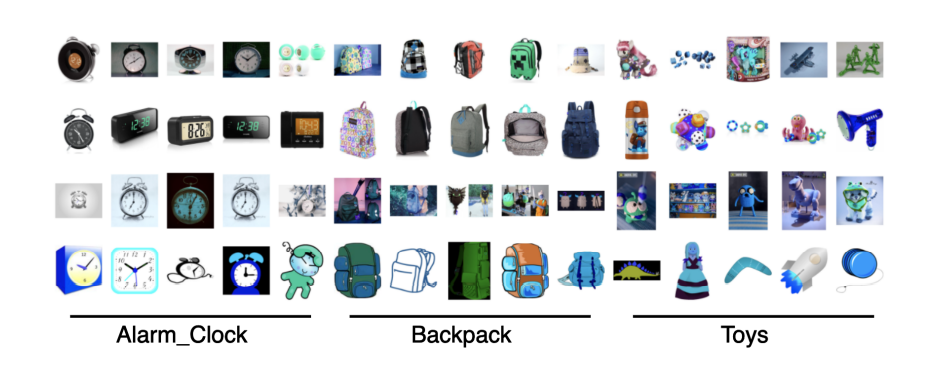
\includegraphics[width=0.95\linewidth]{figure8.jpg}
    \caption{Caption}
    \label{fig:my_label8}
\end{figure}

See the image in figure \ref{fig:my_label9}
\begin{figure}
    \centering
    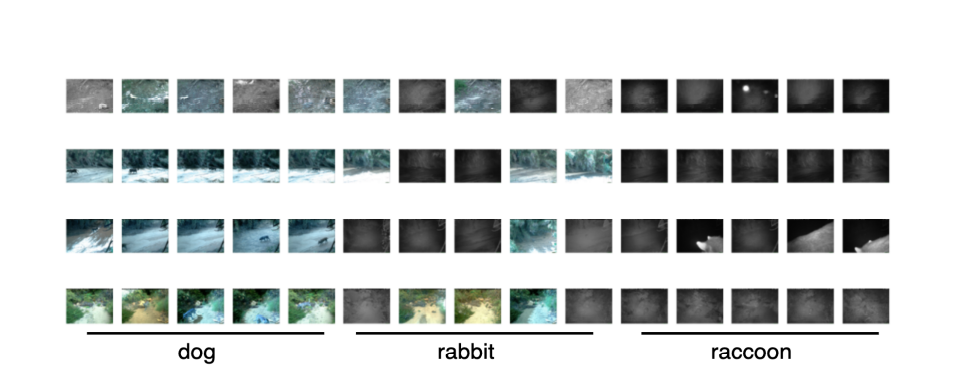
\includegraphics[width=0.95\linewidth]{figure9.jpg}
    \caption{Caption}
    \label{fig:my_label9}
\end{figure}
\section{bibliography}
We used information from this paper \cite{f1} ande this book \cite{giulianotti2009globalization}
\printbibliography
\end{document}

\end{document}
